
\documentclass[BTech]{nitkdiss}
%\documentclass[12pt, a4paper]{report}

\usepackage{amsmath,amssymb,graphicx,color,colortbl}



\title{Real-time 3D sound realization}

\author{Bilal Ali(15EC112)\\Sathwik G S (15EC116)\\ Barun Kumar Acharya (15EC209)\\}
\mentor{Dr. Sumam David}
\date{\today}
\department{Electronics and Communication Engineering}

\begin{document}
\maketitle
\pagestyle{plain}
\pagenumbering{arabic}
\tableofcontents
\listoffigures
\newpage
\begin{abstract}
3D Audio is a generic name that encompasses ways to render audio like in reality and in particular its spatial dimension; it is the capability to produce and perceive sounds in any direction and at any distance. Localization of sounds in physical space plays a very important role in multiple audio-related disciplines.

  Binaural recording is the most commonly used method to provide an immersive sound experience by means of headphone reproduction.The method is based on a time-frequency analysis of the spatial properties of the sound picked up by a simple dual microphone array, assuming source sparseness. 
  Usually  ,  in  order  to synthesize 3D  sound effects  using  binaural  
systems,  we  use  Head-related    transfer    functions    (HRTFs)    to  describe    the    spectral  
filtering    that  occurs  between    a    source  sound  and  the  listener’s  eardrum.  Because  of  the  
characteristics  of  HRTF  some  three-dimensional  effects  in  the  area  of  a  cone  of  confusion  
between front and back directions can be declined. In order to design the system , we derive a large 
set  of  HRTFs  for  different  azimuth  and  elevations  from already present databases and with the help other binaural cues reconstruct the signal to generate the appropriate effect. 
In  this  project  we implement a system for 3D  sound  localization which synthesizes a signal in real-time and aim to achieve with minimal computational complexity. The output sound  quality  is  
evaluated by a subjective listening test. 
\end{abstract}

\chapter{Introduction}
\section{Problem definition } 
We are trying to design a system that will enable the user to realize and virtually locate a sound source heard through headphones. However, the main criteria of this system would be to respond in real-time.
This has become a hot topic in the past few years due to its expanding application in a lot of fields like games, home theaters and human aid systems.  It can improve our experience in some interactive application together with haptic feedback.  
\section{Previous work}
Initial research involved localizing the sound source rather than reproducing it. Several methods have been proposed in different transfer domains to fasten the process of localization.One of most robust methods to in time domain is given by the GCC-PHAT method as discussed by B. Van Den Broeck and A.Bertrand \cite{one} derived from \cite{two}. Moreover it has undergone modifications for more critical situations such as multiple sources, described in \cite{three}.\newline
The amplitude panning method used
in stereo and surround systems today, was invented in 1931 by Alan Blumlein. This method is designed to allow audio sources to be placed at different angular offsets whichs allows instruments to be placed in different positions to build up a sound scene utilising the sine/cosine panning law, or in more advanced cases in surround systems to place sources around a listener in the horizontal plane. The basic concepts 3D sound systems are explained in detail by E. M. Wenzel \cite{four}. General information about the 3D localization of the sound can be realized on the basis of the HRTFs from the source to the right and left ears are discussed by Chong-Jin and Woon-Seng Gan \cite{six}, E, M.Wenzel \cite{four}. The  robustness  analysis,  localization  characteristics,  structural  model  for  binaural  sound  synthesis  and  head  
related transfer functions are discussed in detail by C. Phillip Brown and Richard O. Duda \cite{seven} . HRTF’s (head related transfer functions) allow
localisation of sources in the vertical dimension.It was proposed by Wallach \cite{eight} that dynamic head movements also facilitate the localisation due to head movements which produce variations in inter-aural differences to resolve the position of sources.
Recent research by Ashby et al. (2011) investigated the influence of head rotation on the localisation of elevated sound sources.

In this work we used the HRTFs made available to public by the \textit{Listen project}, which is a shared-cost RTD project in the Information Society Technologies (IST) Program of the European Commission's Fifth Framework Program. In the later stages we have also used HRTFs from the CIPIC Interface Laboratory.
\section{Motivation}
People hear sound in three dimensions and the perception of the spatial aspects of sound has been essential to human survival.Psycho-acoustic researchers have been studying this problem from the view of understanding the functioning of the human hearing system which makes sound
localization possible in the real world, leading to the principles of binaural human hearing. 

With advancements in the field of virtual reality, it becomes really important to make sure that along with visual effects ,the audio is also on the same page (3D effect). Most of the methods existing allow to reconstruct spatialized audio post-processing. We are trying to achieve the whole outcome in real-time. Along with solving the problem of timing constraint , we also want to minimize resource utilization, therefore designing an ASIC as such. In the end, we will try to get a standalone system which gives the user a live surround-audio like experience.

\section{Overview}          
The setup includes a dual microphone arrangement which continuously records and the recorded sound is further filtered. This filtered sound is then played back over headphones. The selection of the filter is based on the location of the sound source w.r.t the center of the microphone setup. Filters are characterized, based on the azimuth and angle of elevation value . \newline
In order to calculate the angle of sound source, we cross-correlate the signals observed on both the microphones and calculate the delay between them. Once this is calculated, appropriate filter is chosen and convolved with the recorded signals. Typically, sounds generated from headphones appear to originate from within the head. In the virtual auditory space, the headphones should be able to “externalize” the sound. Using the HRTF, sounds can be spatially positioned.

\chapter{Background and Implementation}
\section{How do we hear 3D sound with only two ears?}
The auditory system uses the combination of 2 types of information to localize a sound: \textbf{Binaural Cues} (Time and Level) and \textbf{Head Related Transfer Functions} (HRTF).
\subsection{Binaural Cues}
When a sound source is located eccentrically, it is closer to one ear than the other and sound arrives later and weaker at one ear. Time and level difference perception between the two ears provide information about direction. These binaural cues are called Inter-aural Time Difference (ITD) and Inter-aural Level Difference (ILD). They are important for the horizontal localisation. The auditory system evaluates interaural time differences from: (a) Phase delays at low frequencies and (b) group delays at high frequencies. Interaural Intensity Difference (IID) or Interaural Level Difference (ILD) are highly frequency dependent and they increase with increasing frequency. Massive theoretical researches demonstrate that IID relates to the signal frequency f and the angular position of the acoustic source θ. The function of IID is given by:
 \begin{equation}
IID = 1.0 + \frac{f}{1000}^{0.8} \times sin\theta
\end{equation}
\begin{figure}[h!]
  \centering
  \begin{minipage}[b]{0.3\textwidth}
    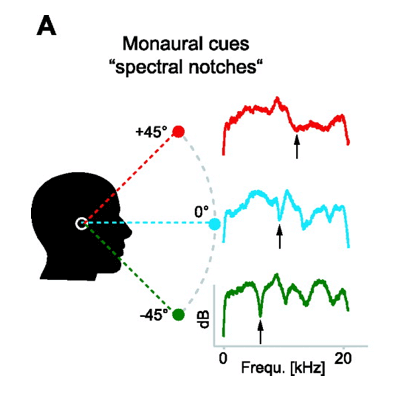
\includegraphics[width=\textwidth]{A}
  \end{minipage}
  \hfill
  \begin{minipage}[b]{0.3\textwidth}
    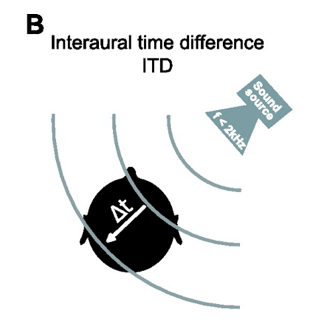
\includegraphics[width=\textwidth]{B}
  \end{minipage}
  \begin{minipage}[b]{0.3\textwidth}
    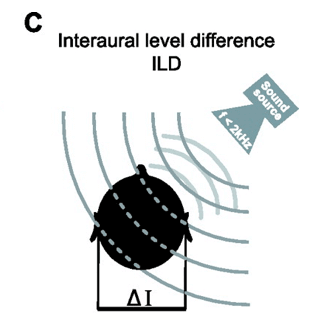
\includegraphics[width=\textwidth]{C}
  \end{minipage}
\end{figure}
For frequencies below 1000 Hz, mainly ITDs are evaluated (phase delays), for frequencies above 1500 Hz mainly IIDs are evaluated. Between 1000 Hz and 1500 Hz there is a transition zone, where both mechanisms play a role.
\subsection{HRTF}
Before reaching the entrance of the ear canal, a sound wave coming from one direction is transformed by the multiple reflections on our body, our face and more importantly our ears. This transformation, called Head Related Transfer Function (HRTF), is different for each direction of sound and has a specific spectral signature for each direction. It is a transfer function, describing how a sound from a specific point will arrive at the ear (generally at the outer end of the auditory canal). The brain has “learned” these signature over time and when it hears a sound with a specific signature, it can find out its direction in its HRTF memory. HRTF is important for vertical localization. A pair of HRTFs for two ears can be used to synthesize a binaural sound that seems to come from a particular point in space. 
\begin{figure}[!tbp]
  \centering
  \begin{minipage}[b]{0.45\textwidth}
    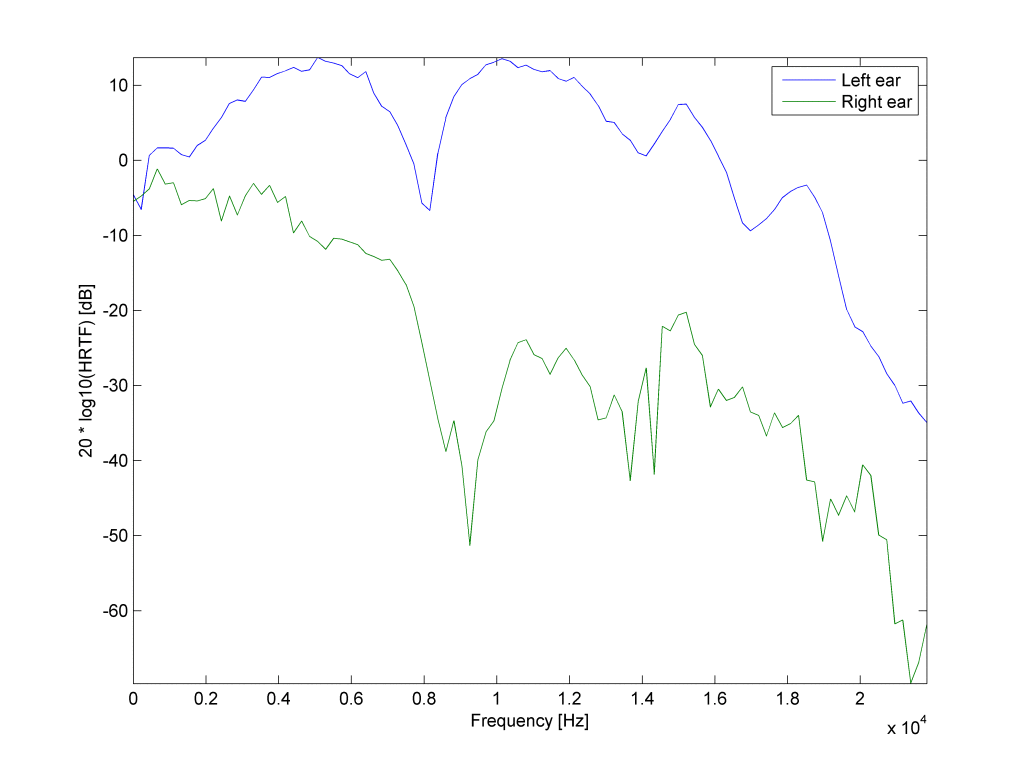
\includegraphics[width=\textwidth]{hrtf_left}
    \caption{HRTF for source to the left}
  \end{minipage}
  \hfill
  \begin{minipage}[b]{0.45\textwidth}
    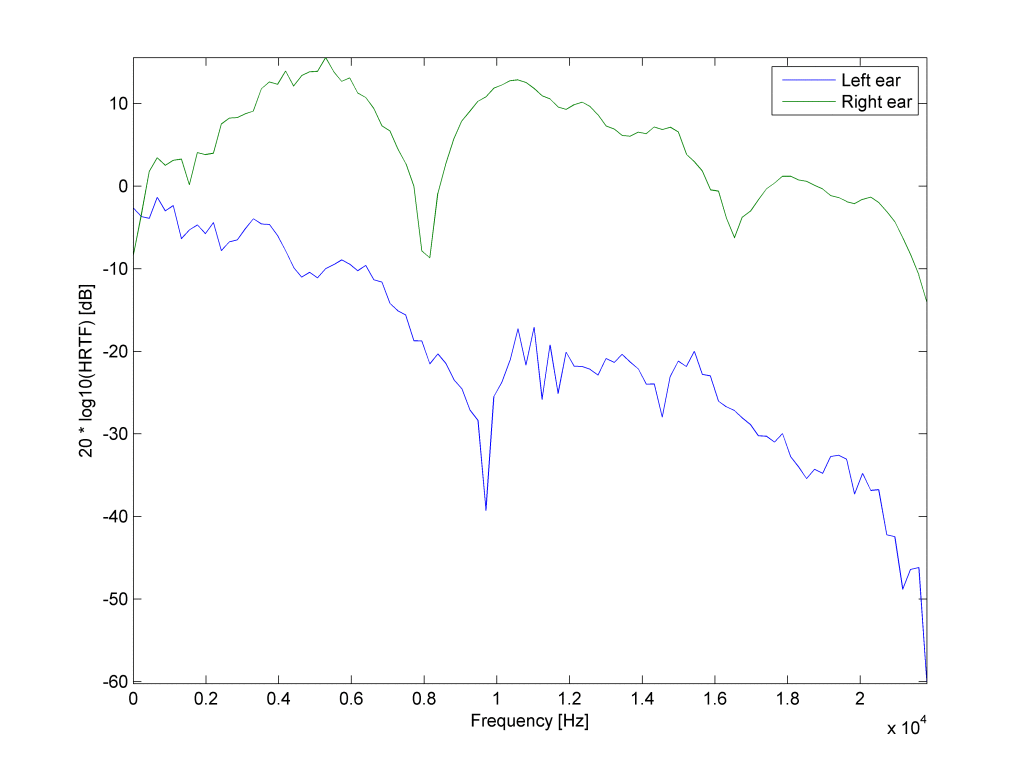
\includegraphics[width=\textwidth]{hrtf_right}
    \caption{HRTF for source to the right }
  \end{minipage}
\end{figure}
HRTFs are typically measured in an anechoic chamber to minimize the influence of early reflections and reverberation on the measured response. HRTFs are measured at small increments of θ such as 15$^{\circ}$ or 30$^{\circ}$ in the horizontal plane, with interpolation used to synthesize HRTFs for arbitrary positions of θ. Even with small increments, however, interpolation can lead to front-back confusion, and optimizing the interpolation procedure is an active area of research. 
\section{HRTF Database}
The area of 3D sound synthesis has been active since a very long time and many research labs have collected the HRIR (Head related impulse response) in well structured environment suitable for audio recordings. Some of these databases are from MIT, UC Davis (CIPIC database) and few privately funded labs. \newline
The database is maintained based on recordings from different subjects (with varying anthropometric data). Each subject is equipped with a pair of microphones and is made to sit in an anechoic chamber. Test sounds are played and the perceived signals on each ear is recorded. These sounds are played from different azimuthal as well as elevated angles. Some of the database includes anthropometric measurements for use in HRTF scaling studies.
\begin{figure}
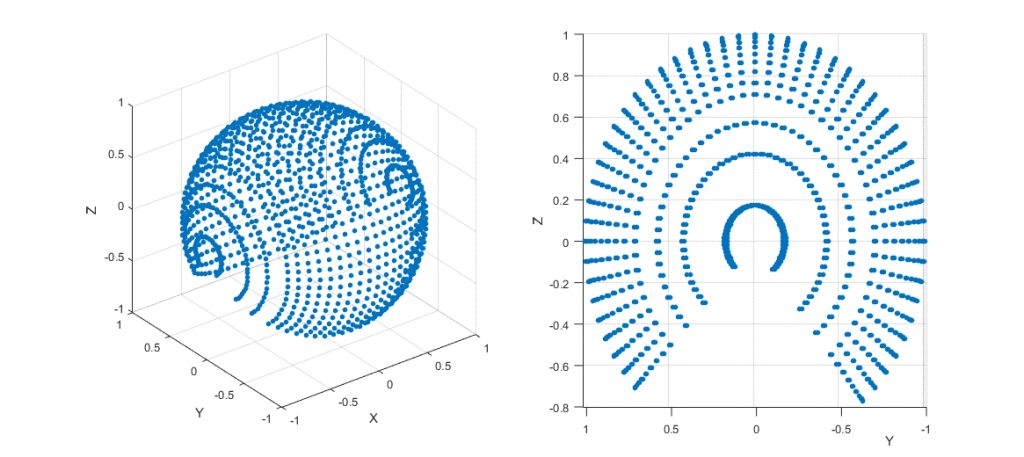
\includegraphics[width = \textwidth]{data_points}
\caption{Visualization of points at which HRIR from CIPIC are recorded.}
\end{figure}
\section{The setup}
%Record with 2 microphones
The system we plan to design receives audio input , gets filtered and is played back through headphones with 3D-like effect. \newline
For collecting audio samples, we recorded audio input using 2 microphones separated by 20cm (approximate distance between two ears). We used the National Instruments Data Acquisition module to simultaneously record the input from 2 microphones at 44.1 kHz sampling rate. The recorded data were passed as text files to MATLAB environment for further processing .This was as far as testing the unit was concerned. Later, during the actual test of the entire design we used MEMS Microphones (ADMP401) to acquire audio signals. 
%correlation & angle resolution
\subsection{MATLAB}
The hrtf database was loaded along with the audio file. Cross-correlation between input received at left microphone and the input received at the right microphone was performed. Based upon the results of cross-correlation , we get the time difference of arrival of audio input at the left microphone and the right microphone. Based on this time difference, we can predict the azimuthal and spatial information of the audio source. 
\begin{equation}
\tau = \frac{Max(S_{L} * S_{R}) - Signal length}{Sampling Frequency} 
\end{equation}
where '*' operator denotes the cross-correlation operation on left and right microphone signals. 

\begin{equation}
Sin\theta = \frac{\tau c}{d}
\end{equation}
where c is speed of sound in air , d is 20cm, $\theta$ is azimuthal angle .

%Software
Based on the above values, a particular HRTF filter was chosen and convolved with the input. The output we observed showed features clearly indicating spatial properties. In the same way we tested for different azimuthal angles using its corresponding HRTF filter coefficients. This experiment was done solely to understand and verify the functionality of the filters. 
 % DIGITAL DESIGN 
\subsection{Digital design - Version 1.0}

This section explains the first version of the digital design and implementation of the basic functionality of realizing 3D audio effect, which was done during the early stages of the project. After testing the following design and realising some improvements, changes were made and restructured in \textit{Version 2.0} mentioned later in this section.

\begin{figure}[h!]
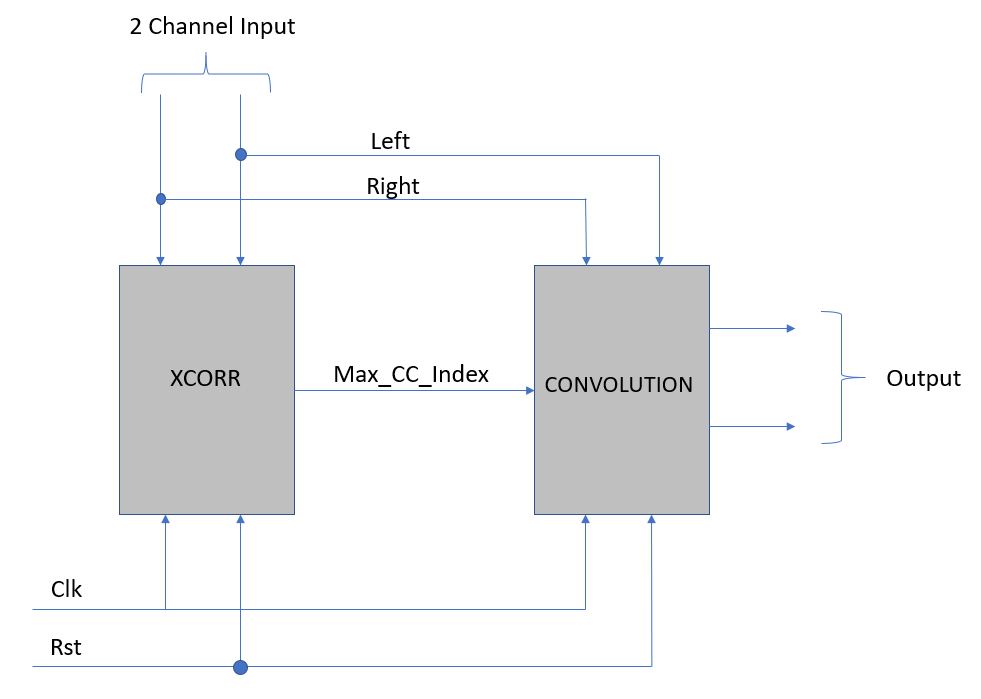
\includegraphics[width = \textwidth, height = 8cm]{Architecture_main}
\caption{Overall Design}
\end{figure}

In order to reduce the complexity but maintaining the quality of filters , the filter coefficients were down-sampled from 512 (originally available in the database) to 64. The sampling rate of audio input, assumed to be 44.1 kHz. \newline


The overall flow of data is as follows:- 
\begin{itemize}
\item 2 channel 16 bit input is given to the 'xcorr'(Cross Correlation) unit 
\item This unit collects 30 data samples and finds the delay between the two signals by cross-correlating them.
\item Using this delay, input data samples are convolved with appropriate filters (indexed by the delay) 
\item The resultant 2 channel output is played back
\end{itemize} 
\subsubsection{Data format}The RTL design assumes all kinds of data to be in the following format : 
\begin{itemize}
    \item Inputs/Outputs must be signed 16 bits 
    \item Each value should be in 1.15 format where MSB bit is the sign bit and remaining 15 bits are the fractional bits
    \item Range of values should be from -1 to 1 
\end{itemize}

\subsubsection{MAC Unit}
This is the most important arithmetic unit of the overall design. The following Figure \ref{fig : mac_unit} shows the data flow. 
\begin{figure}[h!]
\centering
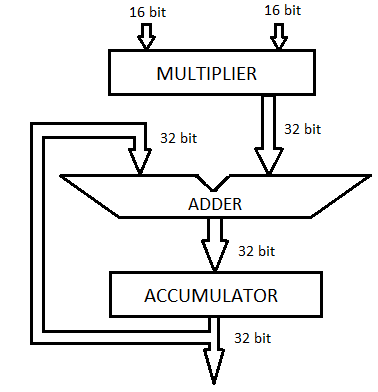
\includegraphics[width = 5cm, height = 6cm]{mac}
\caption{MAC Unit}
\label{fig : mac}
\end{figure}
It uses only \textbf{One} multiplier (16 bits) and keeps accumulating the resultant 32 bit iteratively. The final result is stored in a register, Figure \ref{fig : mac}. One must be careful with the bitwidth of the result and truncate proper bits. 

\textit{\textbf{Note:}} MAC output must truncated to 16 bits, else will lead to miscalculation in further stages. 

\subsubsection{XCORR}
The main function of  this module is to cross correlate between any two signals. Since the setup involves 20cm between the two recording devices and assuming speed of sound to be 343 m/s, the maximum delay possible comes out to be around \textbf{27} samples. Therefore, the signals correlated are of length 30 samples.  
\begin{figure}[h!]
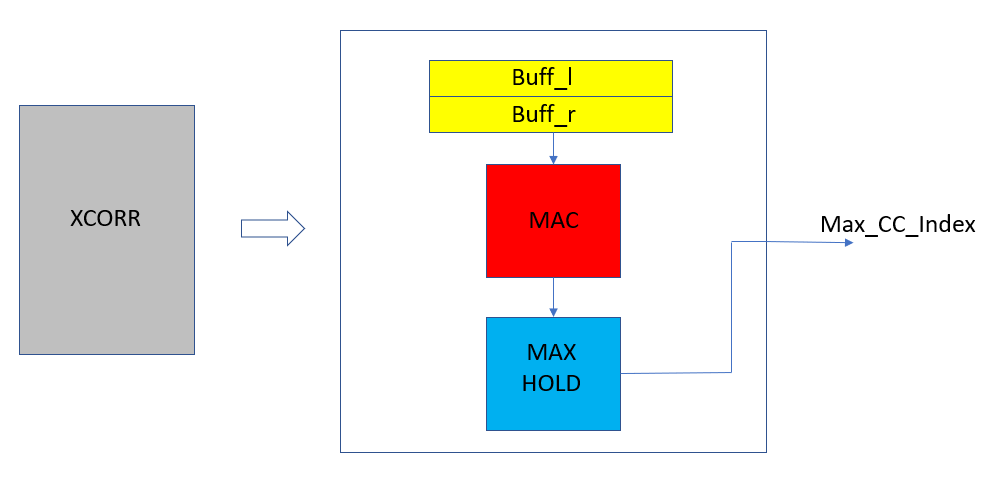
\includegraphics[width = \textwidth]{xcorr}
\caption{XCORR Module}
\label{fig: xcorr_module}
\end{figure}
Initially, the buffers of both the channels collect those 30 samples and pass it on to the \textbf{MAC} unit. Here, the signals are multiplied and added. One of the buffer is shifted and the process is repeated until the buffer slides out, Figure \ref{fig : correlation}. 
\begin{figure}[h!]
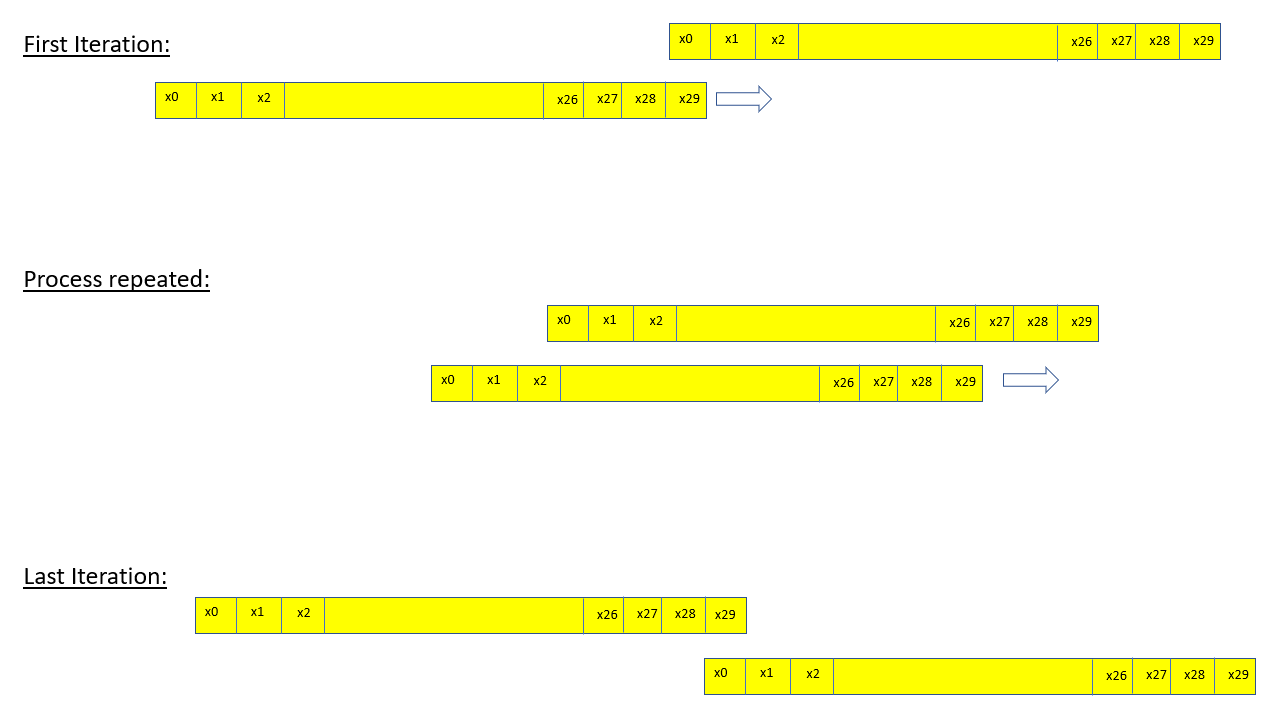
\includegraphics[width = \textwidth, height = 9cm]{slide}
\caption{Correlation operation -  at each iteration the corresponding elements are multiplied and added}
\label{fig : correlation}
\end{figure}                
The 'Max-hold' unit keeps track of the maximum value of the MAC unit. It updates whenever a new maximum is found. After completion of the process, the index of shift corresponding to maximum MAC value it passed as the output.

\textbf{Calculation of clock speed required:} Given that the sampling rate = 44.1 kHz, at the end of acquiring 30 samples within a sample period there must be 59 shifts (length of cross-correlation output) with 30 MAC operation in each shift. Thereby giving rise to clock requirement which is 59x30 = 1770 times faster than 44.1 kHz. This implies clock speed required is = 78 MHz.


\subsubsection{Convolution and Filter Bank}
This module performs 2 tasks; selecting appropriate filter from a filter bank and convolving the same with input data samples. 
\begin{figure}[h!]
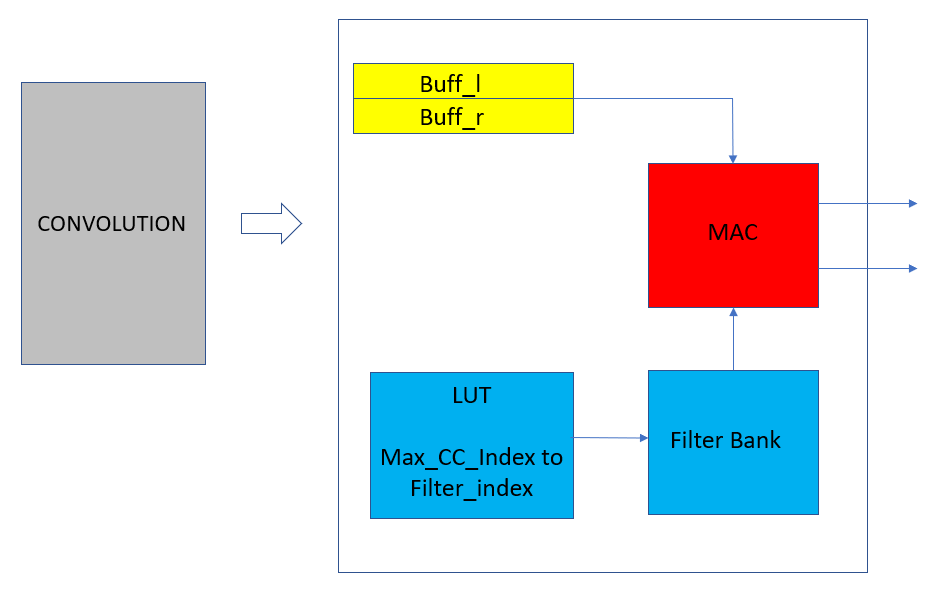
\includegraphics[width = \textwidth, height = 10cm]{conv_filter}
\caption{Convolution Module}
\end{figure}
The buffer lengths are once again 30, since these are the same samples whose cross-correlation is being computed. But, each filter corresponding to a certain azimuthal angle has \textbf{64} coefficients, therefore we would have to use \textbf{34} samples of previous frame. 
\begin{figure}[h!]
\centering
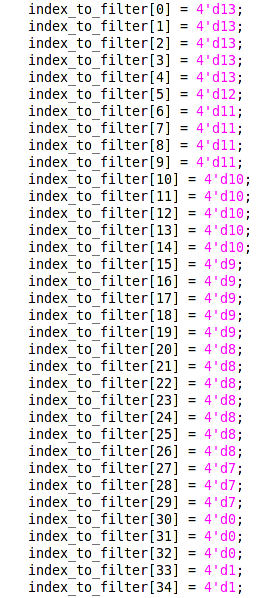
\includegraphics[width = 4cm, height = 7cm]{index1}
\caption{Maximum Correlation index to Filter Index Mapping} 
\label{fig : Index mapping}
\end{figure}
\newline In order to choose appropriate filter, the index from the \textbf{xcorr} module is mapped accordingly to filter index, see Figure \ref{fig : Index mapping}. 

We observe that as the delay increases, even a small change in it causes change in filter selection. This implies that around midway the resolution is highest. After selecting the filter, the coefficients are then convolved with input samples (of length 30) + past 34 samples to give  the output. \newline The filters used are derived from the database, of which filters corresponding to only 0$^{\circ}$ elevation are used here and there are \textbf{13 different} azimuthal angles each with 64 coefficients. All these coefficients are stored in banks of registers and indexed accordingly. 

\subsection{Digital design  - Version 2.0} \label{version2}

This section will include all kinds changes made after checking the output of the previous design in real time. The following problems were faced and needed to be addressed: \begin{itemize}
    \item Filters were changing too fast, resulting in not-so-pleasant output
    \item Given the output sample rate, the computational main clock speed required was too high
    \item Audible glitch during transition from one filter to another 
\end{itemize}

The filters were then changed to 100 coefficients \textit{(Initially 200 length -- CIPIC HRTF Database)}. This database had more number of filters for different directions. In the azimuthal sense, it has 25 different filters. Although the MAC unit remains the same , changes were made in the \textbf{XCORR and Convolution unit}.

\subsubsection{Modified XCORR}

Previously, only 30 samples were used to correlate and this was done on every 30 sample data frame. This sometimes led to random angles due to possible presence of noise samples more than the actual audio/speech samples. Considering the sampling rate of 44.1 kHz, 30 samples = 0.68 ms which is extremely short, hence it is required to compute the cross-correlation at a slower rate with longer frames. 

\begin{figure}
    \centering
    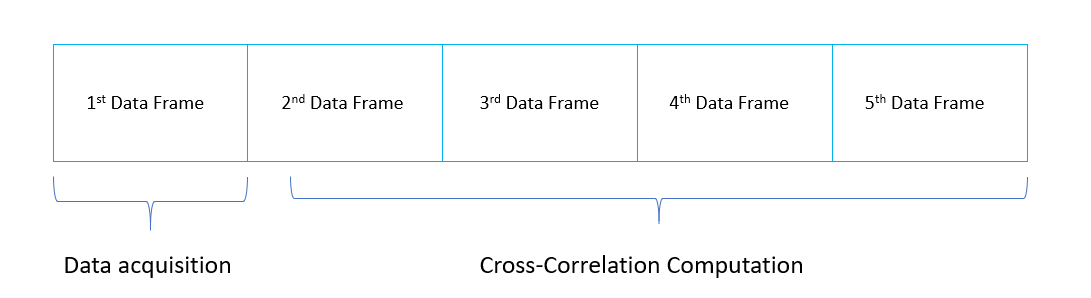
\includegraphics[width = \textwidth, height = 5cm]{modified_xcorr.png}
    \caption{Modified XCORR}
    \label{fig:modxcorr}
\end{figure}
\begin{figure}[h!]
    \centering
    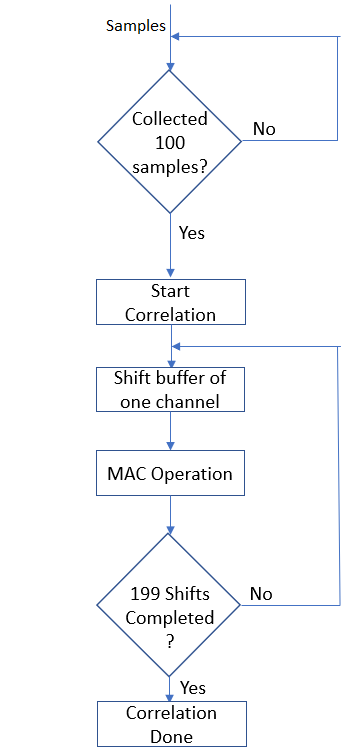
\includegraphics{xcorr_flow.png}
    \caption{Dataflow for cross-correlation}
    \label{fig:dataflow}
\end{figure}

The modified XCORR unit now considers a data frame of 100 samples long illustrated in Figure \ref{fig:dataflow}. Unlike the previous design which \textbf{collected samples} and computed the output \textbf{before} the next data frame resulting in higher clock speed requirement, the new design now collects 100 samples and computes the output in the time period of next 400 samples as shown in Figure \ref{fig:modxcorr}. In other words, cross correlation of \textbf{100 samples but of every 5th data frame}, thus computing period of \textbf{4 data frames} resulting in relaxed clock speed requirements. These changes will make sure that the rate of correlation is decreased and the clock speed required is also significantly \textbf{reduced}. 

\subsubsection{Modified Convolution unit}

This unit will now deal with convolving 100 data samples with a corresponding filter. The changes to be made here should tackle the issue of audible glitch while transition between filters. Now that the cross-correlation module (XCORR) gives out new index every 5th frame (5*frame.lengths = 11.3 ms), it is important to make sure that the valid cross correlation index is used to choose the appropriate filter.

\begin{figure}[h!]
    \centering
    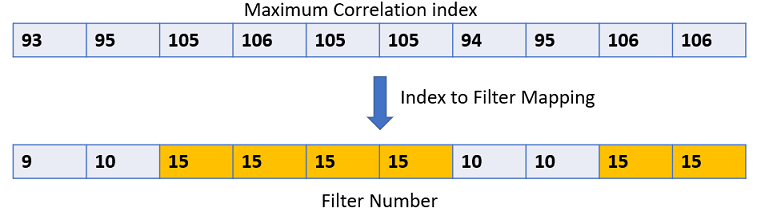
\includegraphics{index_2_filter.png}
    \caption{Choosing filter}
    \label{fig:index2filter}
\end{figure}

In order to choose the valid filter, we then keep track of \textbf{past 10} cross correlation indices mapped to corresponding filter as shown in Figure \ref{fig:index2filter}. The filter which occurs the \textbf{most amount} of times is then chosen as the new filter (in this case shown filter 15 is chosen) and brought into the computation as shown in the following section. The index to filter mapping was redone to account for the new cross-correlation indices. This essentially means that there could be a change in filter in about \textbf{every 110 ms} which can still account for any change in location of the sound source. 

\begin{figure}[h!]
    \centering
    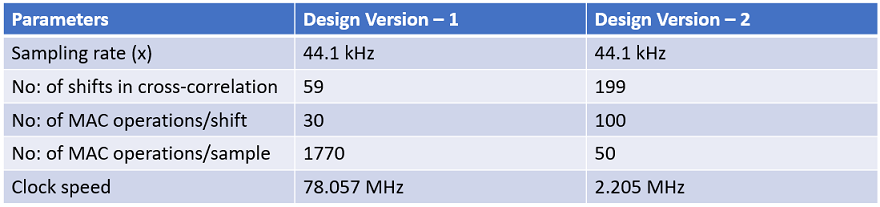
\includegraphics[width = \textwidth, height = 4cm]{parameters.png}
    \caption{Comparison}
    \label{fig:comparison}
\end{figure}

\subsubsection{Live Convolution with time varying FIR filters}
Amid the procedure of filter change, rather than totally supplanting the filter one should let the convolution with the present filter to get finished and yet begin convolving with the latest one. This process requires \textbf{2 convolution units} operating at the same time.
\begin{figure}[h!]
\centering
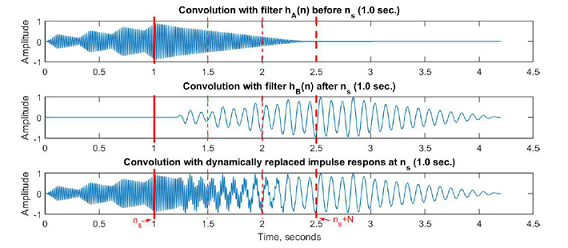
\includegraphics[width = \textwidth, height = 7cm]{update.png}
\caption{Filter change at T=1s}
\label{fig : live}
\end{figure}
\begin{figure}[h!]
    \centering
    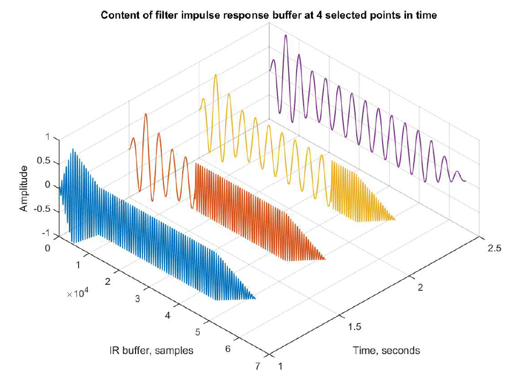
\includegraphics{coeff_update.png}
    \caption{Filter Coefficient Update}
    \label{fig: coeff_update}
\end{figure}
There is another approach to accomplish the equivalent yet utilizing just 1 convolver \cite{live}. During the exit phase of the present filter a portion of the initial coefficients don't add to the outcome, however has a job for the latest filter. In a way the filter buffer should be loaded up with \textbf{partial commitments} from both the filters, illustrated in Figure \ref{fig: coeff_update}.
For each sample update in the buffer to be convolved with, the coefficients are updated at the same time.

This approach is equivalent to the using 2 convolvers but the advantage being, requirement of only \textbf{1 multiplier unit} at a time. 

\subsubsection{Smooth Transition}
To avoid audible glitches while transition we slowly introduce the new filtered output into picture rather than just abruptly appending it. This can be done by crossfading the output of a particular data frame with the previous filter and fade in the output with the current filter, as shown in Figure \ref{fig:crossfade}. Standard fading techniques such as linear, square-root, sin-cos etc can be used and \textbf{dynamically} generated without having to store them, as shown in Figure \ref{fig:fadegen}. Depending on fading in or fading out, values are incremented or decremented respectively. This value is then multiplied with corresponding filter outputs as shown in Figure \ref{fig:crossfade}. 

\begin{figure}
    \centering
    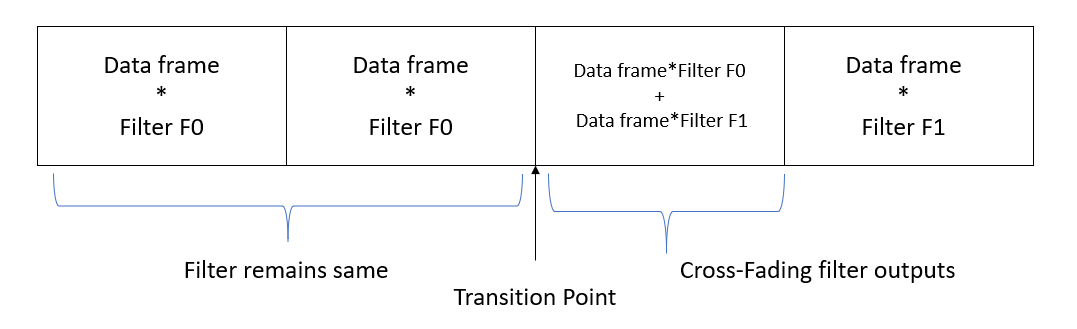
\includegraphics[width = \textwidth, height = 5cm]{Crossfade.png}
    \caption{Transition between filters}
    \label{fig:crossfade}
\end{figure}

\begin{figure}[h!]
    \centering
    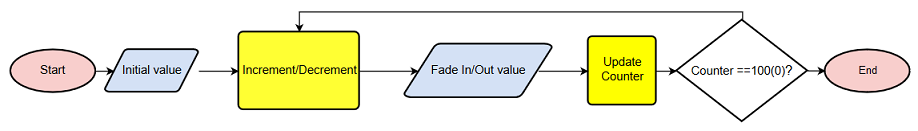
\includegraphics[width = \textwidth]{fade_gen.png}
    \caption{Fade In/Out Generator}
    \label{fig:fadegen}
\end{figure}



All these changes resulted in overcoming the problems faced by the previous design. 

\section{FPGA Implementation}
In order to test the design and check its functionality in real time \textbf{Nexys 4 DDR Artix -7 FPGA (now renamed as Nexys A7)} which has enough resources to accommodate our design requirements was used.

\subsection{Input}
The design requires a two channel input essentially coming from two microphones separated by about 20cm. Here, we have used \textbf{ADMP401 MEMS Microphones} which is omnidirectional, analog output, low power and has flat frequency response from 100Hz to 15 kHz suitable for near and far field applications. We must convert the incoming analog signals from the microphones to digital form using an \textbf{ADC}.

\begin{figure}[h!]
    \centering
    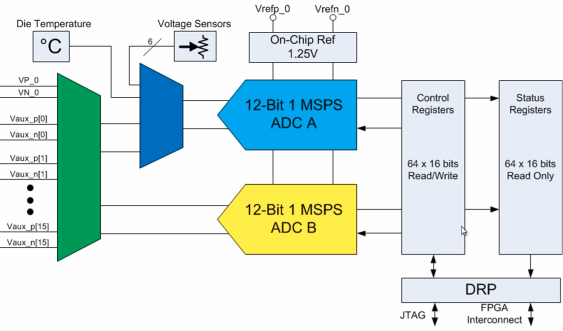
\includegraphics[width = \textwidth]{XADC.png}
    \caption{XADC Interfacing}
    \label{fig:xadc}
\end{figure}
The chosen FPGA board has an on-chip analog-to-digital converter (XADC), which is a \textbf{12-bit dual channel ADC} with a maximum sampling rate \textbf{1 Mega-samples per second (1MSPS)}. From Figure \ref{fig:xadc}, we can see that the XADC supports upto 16 auxillary channels along with a dedicated analog channel with better sampling rate. The converted digital output of each channel is stored in status registers. The register address for Control and Status registers are mentioned in the Figure \ref{fig:xadcreg}. For example, choosing auxillary channel 10 would result in storing the values in register with address \textbf{0x1A} . This project requires sampling and conversion of two analog channels, therefore XADC must be configured in \textbf{\textit{Channel sequencer}} mode where each channel is sampled one after another in a loop.  
\begin{figure}[h!]
    \centering
    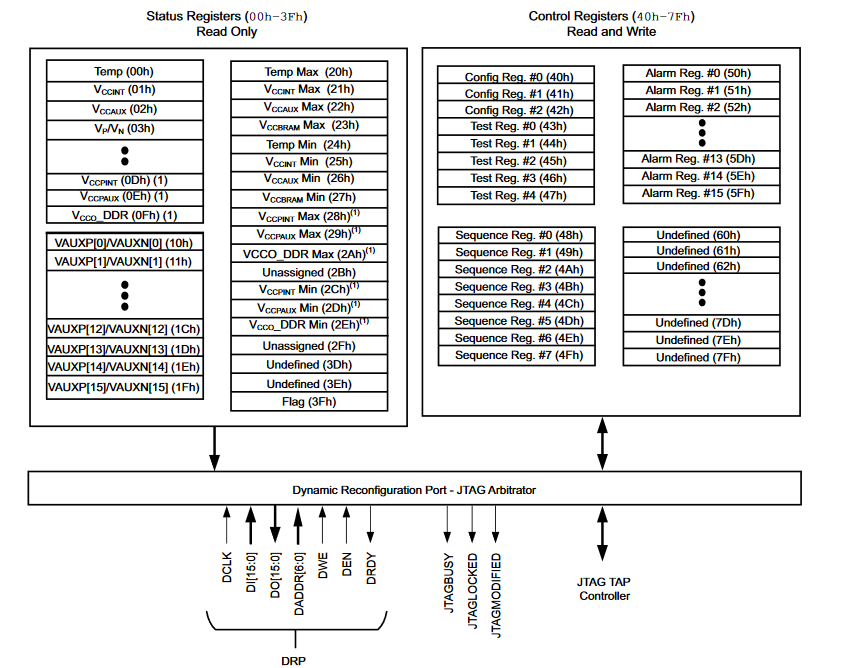
\includegraphics{XADC_Registers.png}
    \caption{XADC Register Interface}
    \label{fig:xadcreg}
\end{figure}
\begin{figure}[h!]
    \centering
    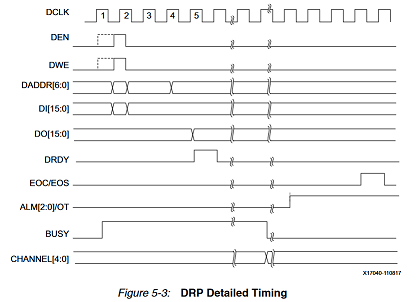
\includegraphics[height = 6cm]{drp_timing.png}
    \caption{Detailed timing of events}
    \label{fig:drptiming}
\end{figure}

However, the output from the module is a 16-bit data which just appends 4 bit zeros (in LSB) to the converted 12 bit value. As seen from Figure \ref{fig:drptiming}, the converted value its latched into status register only when \textbf{DRDY} signal goes high. Hence, when it is under multiple channel mode \textbf{DRDY} signal and register address specified in \textbf{CHANNEL[4:0]} signal must be used together to retrieve valid converted data values which is available on \textbf{DO[15:0]} wire. Xilinx's Vivado design suite which helps in programming this FPGA has wizards to configure the \textbf{XADC} settings and get the instantiation template to use with our design (code). 
\textit{\textbf{Note:} XADC requires the input peak-peak voltage to be at max 1V, potentiometer can be used to tune the voltage levels accordingly}

\subsection{Importing Design}
The previously designed modules were imported here (Vivado design suite) with ease. Proper clock rates and bit-widths of input/output were checked carefully which are usually the common sources of error while implementing. 
\begin{figure}[h!]
    \centering
    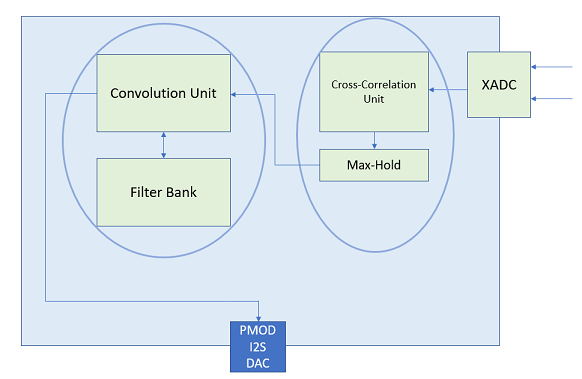
\includegraphics{fpga_layout.png}
    \caption{Block Representation}
    \label{fig:fpgablock}
\end{figure}

\begin{figure}[h!]
    \centering
    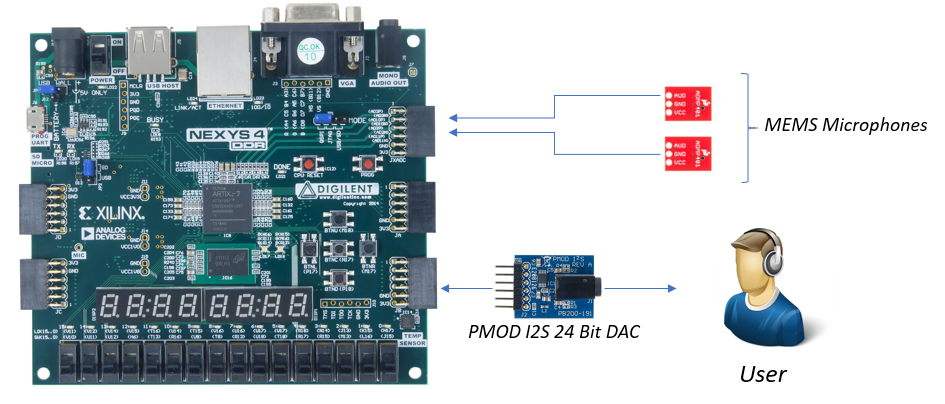
\includegraphics[width = \textwidth, height = 7cm]{fpga_implementation.png}
    \caption{Setup}
    \label{fig:my_label}
\end{figure}
\subsection{Output}
The overall processed output of the entire design consists of 2-channel 16 bits data which needs to be converted to equivalent analog form and be heard through headphones. In order to implement this, DAC (Digital to Analog Conversion) unit is required. Hence, we have used an external \textbf{16-24 bit Stereo Pmod i2S DAC} module. It follows the \textit{I2S} protocol which is typically used when dealing with audio signals. Thereby, we need to also introduce a block in our design code to include this transmission process. 

\begin{figure}[h!]
    \centering
    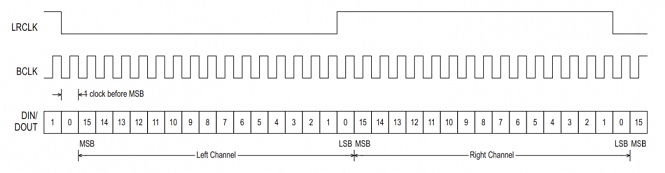
\includegraphics[width = \textwidth, height = 4cm]{i2s.png}
    \caption{I2S Protocol}
    \label{fig:i2s}
\end{figure}

\begin{figure}[h!]
    \centering
    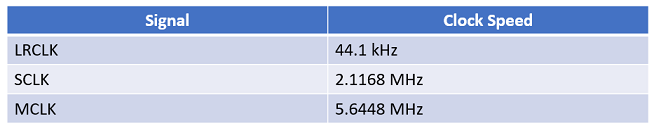
\includegraphics{i2sclkspeeds.png}
    \caption{Clock speed of different signals involved in I2S transmission}
    \label{fig:i2sclk}
\end{figure}
Xilinx's clocking wizard can be used effectively to get clock speeds ranging from 4 Mhz to 100 Mhz and later directly instantiate the same with ease. Here, in order to get clock speeds lesser than 4MHz we used clock dividers from the nearest multiple near 4MHz and derived it. From Figure \ref{fig:i2sclk}, for example \textbf{\textit{SCLK}: clock speed upto 4.2336 MHz} was generated from clock wizard and then halved manually. Typically, sending the data greater than sampling rate is advised since in that case you won't be missing any data to be transmitted. The PMOD module comes with a 3.5mm headphone jack which can be plugged in to listen to the output. 



\chapter{Testing and Observations}
Here are some of the observations, which were observed while experimenting with different audio samples and different HRTF filters.  
\section{Observation}
\subsection{Angle resolution}
When the signals were correlated to get the difference in time of arrival for both microphones, for source angle range of 0$^{\circ}$ - 90$^{\circ}$ the number of distinct values (for Sampling rate = 44.1 kHz) was 26.
\begin{equation}
0^\circ - 90^\circ = 26 (values)
\end{equation}

\subsection{Panning}
Panning is the spread of a monaural signal in a stereo or multi-channel sound field. Here, we realize different directions of sound source by changing the filters accordingly. The resultant effect when heard will be equivalent to as if the source is moving around the head. 
\begin{figure}[h!]
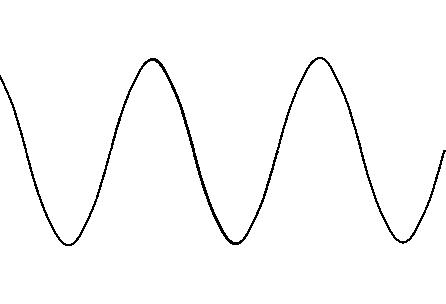
\includegraphics[width = \textwidth, height = 5cm]{sine}
\caption{Input: Sine wave of 1kHz}
\end{figure}
\begin{figure}[h!]
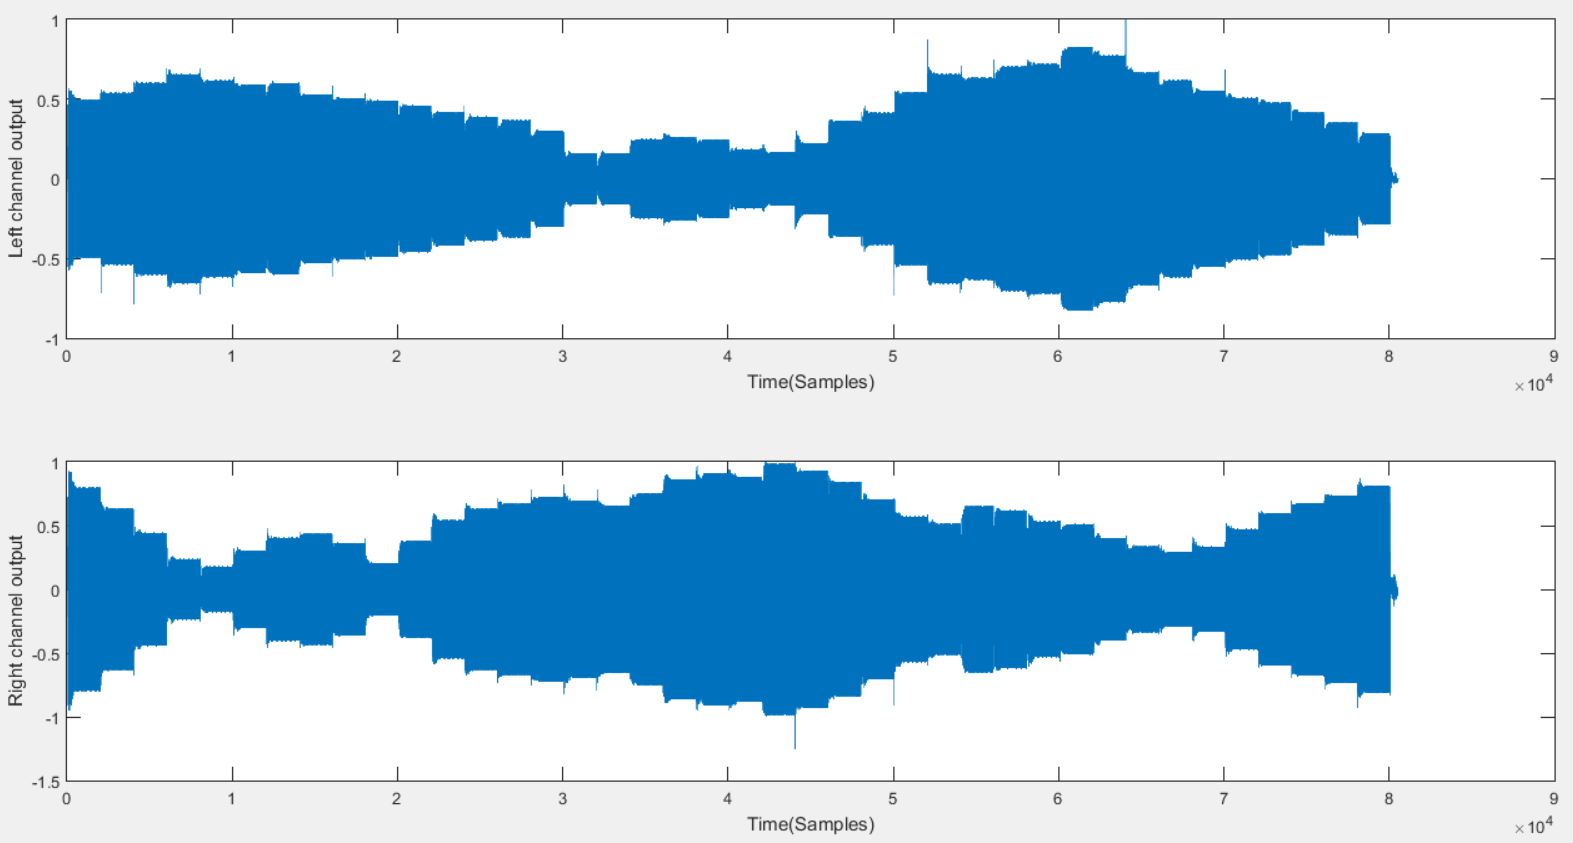
\includegraphics[width = \textwidth, height = 7cm]{output_sine}
\caption{Output: After panning}
\end{figure}
This test was done in MATLAB to realise the functioning of HRTFs. 
\subsection{Testing Design}

During the FPGA implementation we tried to generate the effect of \textbf{Panning} as a part of testing the filter output. This was implemented with, the user being able to select the angle of source and realise the effect. This test turned out to be successful with no problem in the output. Along with that , the \textbf{actual design} was also imported which detected proper \textbf{angle of sound source}. However, the design sometimes struggled under multiple sound sources. This can be said as one of the drawback of this design. 

\begin{figure}
    \centering
    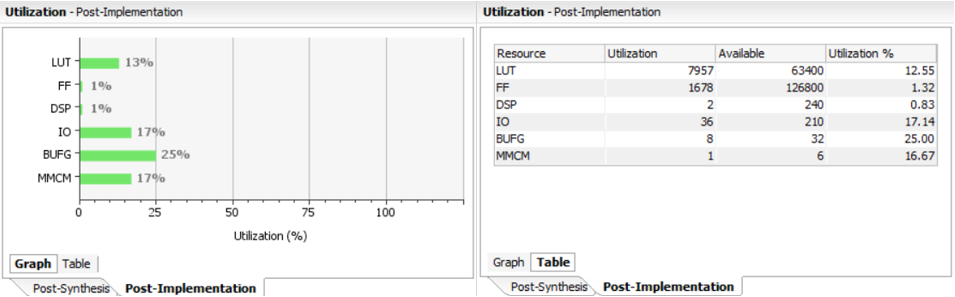
\includegraphics[width = \textwidth]{utilisation.png}
    \caption{Resource Utilization}
    \label{fig:utilise}
\end{figure}

From the resource utilisation, Figure \ref{fig:utilise} we observed that most of the resources were taken up by storing the filter coefficients. If there was some kind of external memory interfacing used, the utilisation would have been significantly reduced. But as far as the quality and realisation of 3D sound is concerned the output was clear and as expected.


\chapter{Conclusions}

\section{HRTFs}
After working with such filters we can easily say that HRTFs are a convenient way to realise the simulated effect of 3D surround sound. The change of filters differing in the azimuthal angle indeed causes a large difference in the audio output. Where as , change in elevation didn't cause much of impact. This can also be because of the \textit{non-individualised} filter response. This means that HRTFs usually works the best when the filter responses are actually recorded with one's own facial structure. This is mainly because of the greater impact of parameters such as \textit{ear shape, size, torso} matters in the overall hearing response. It was also observed that the filter length could be as low as \textbf{64}, below which resulted in compromise in audio quality. We always aimed to have the number of filter coefficients as \textbf{low} as possible to reduce the number of \textbf{MAC operations} but also wanted to have a \textbf{sharp} frequency response. A filter length of \textbf{100} proved to be optimal in its performance.   

\section{Analysis of MATLAB implementation}

MATLAB being a handy tool helped in quick design checks and simulation. Although any kind of testing there would be post-processing but, helped in giving more insights about the process in terms of \textbf{plots, spectrum} etc. 

In order to verify the output of the RTL design, scripts were written to mimic the exact process here which accelerated the process of testing. The only difference being that the MATLAB was working on \textbf{floating point} represented numbers where as in the hardware side all sorts of data were represented in \textbf{fixed point format}. 

\section{Analysis of RTL Design}

As mentioned before during the course of this project there were 2 versions of RTL design, which was the resultant of testing them in real time and realising the shortcomings. 

\subsection{Analysis of Design - Version 1.0}

The \textit{Version 1.0} had the following design characteristics:

\begin{itemize}
    \item Correlation of 30 samples
    \item Calculating delay in consecutive data frames
    \item 64 tap filters 
    \item 13 different filters for particular elevation 
\end{itemize}

The issues with this design as mentioned in section \ref{version2} had to be addressed and resolved. Although this design required less number of computations but, they had to be done in a quick interval of time and was idle for the most part of it. Hence not completely utilising the time available for calculation. This was one of the main reason giving rise to higher clock speed requirement. 

\subsection{Analysis of Design - Version 2.0}

After learning that the rate of correlation and calculation of angle of sound source can be relaxed, changes were made and represented in \textit{Version 2.0}. The design characteristics are :

\begin{itemize}
    \item Correlation of 100 samples
    \item Calculating delay in every \textbf{5th} data frame
    \item Computing period of \textbf{4} data frames
    \item 100 tap filters
    \item 25 different filters for particular elevation 
\end{itemize}

This design resulted in better control for selection of filters. One of the main aspects of this architecture was to carefully transit between filters producing smooth output. This was explained in detail in section \ref{version2}. The overall output observed was as expected with \textbf{proper angle of sound source detection and change of filters accordingly}. 


\section{Final Inference}

Given that the aim of this project was to enable the user to \textbf{realise 3D surround sound} only through a pair of earphones, the designed system serves the purpose and functions in \textbf{real time}. Based on subjective listening test it was verified that the user was indeed able to locate and the visualise the sound source \textbf{emerging from a particular direction}. 

\section{Future Work}

There are certain drawbacks in this system which needs to be looked upon. The following can be the upgrades or modifications: 
\begin{itemize}
    \item Modify the system to include the presence of multiple sound sources
    \item Real time tracking of head movements to dynamically update the filter selection
    \item Emphasize the effect of elevation
\end{itemize}

\begin{thebibliography}{9}
\bibitem{one}B. Van Den Broeck, A. Bertrand, P. Karsmakers, B. Vanrumste, H. Van hamme and M. Moonen, "Time-domain generalized cross correlation phase transform sound source localization for small microphone arrays," 2012 5th European DSP Education and Research Conference (EDERC), Amsterdam, 2012, pp. 76-80.
\bibitem{two}C. Knapp, G. Carter, "The generalized correlation method for estimation of time delay,''IEEE Transactions on Acoustics Speech and Signal Processing, vol. 24(4), pp. 320-327, 1976.
\bibitem{three}B. Kwon, Y. Park and Y. Park, "Analysis of the GCC-PHAT technique for multiple sources," ICCAS 2010, Gyeonggi-do, 2010, pp. 2070-2073.
\bibitem{four}E. M. Wenzel, “Localization in virtual acoustic displays,” Presence, vol. 1, pp. 80– 107, Winter 1992.
\bibitem{live} Brandtsegg, $\Phi$.; Saue,S. Live Convolution with Time-Variant Impulse Response , DAFx-17, September 2017.
\bibitem{six}Chong-Jin Tan and Woon-Seng Gan, “User-defined spectral manipulation of HRTF for improved localization in 3D sound systems,” IEEE electronic letters, vol. 34, pp. 2387-2389, Dec. 1998. 
\bibitem{seven}C. Phillip Brown and Richard O. Duda, “A Structural Model for Binaural Sound Synthesis”, IEEE Transactions on 
speech and audio processing, VOL. 6, NO. 5, 1998
\bibitem{eight}Hans Wallach, "The role of head movements and vestibular and visual cues in sound localization", Journal of experimental psychology, Vol. 27 (4)
\end{thebibliography}

\end{document}
